\section{Tracking performance and resolution}\label{sec:tracking}
\sectionstate{requote}{\texttt{mx\_june\_wft/FLEET\_DIGEST.md} (r06, reproduced 10-09, C1); \texttt{sps\_beam\_test\_26/analysis/spatial\_resolution}}
\intent{What the chambers deliver with the reconstruction of the companion paper~\cite{paperII}: angle and position
on cosmics for all five chambers, and the intrinsic resolution of det4 in the beam with the reference fitted out.}

\subsection{Cosmic rays}
\tbw{$\sigma_\theta$ = \requote{1.15--2.51\textdegree}, better than hits on every plane; position residuals; bias; per chamber.}
\analysis{D1}{re-quote from r06}
\askDylan{C2: freeze r06 as it is, or the per-plane c2/c1 (pvy95 re-pass, staged)?}
\begin{figure}[t]
  \centering
  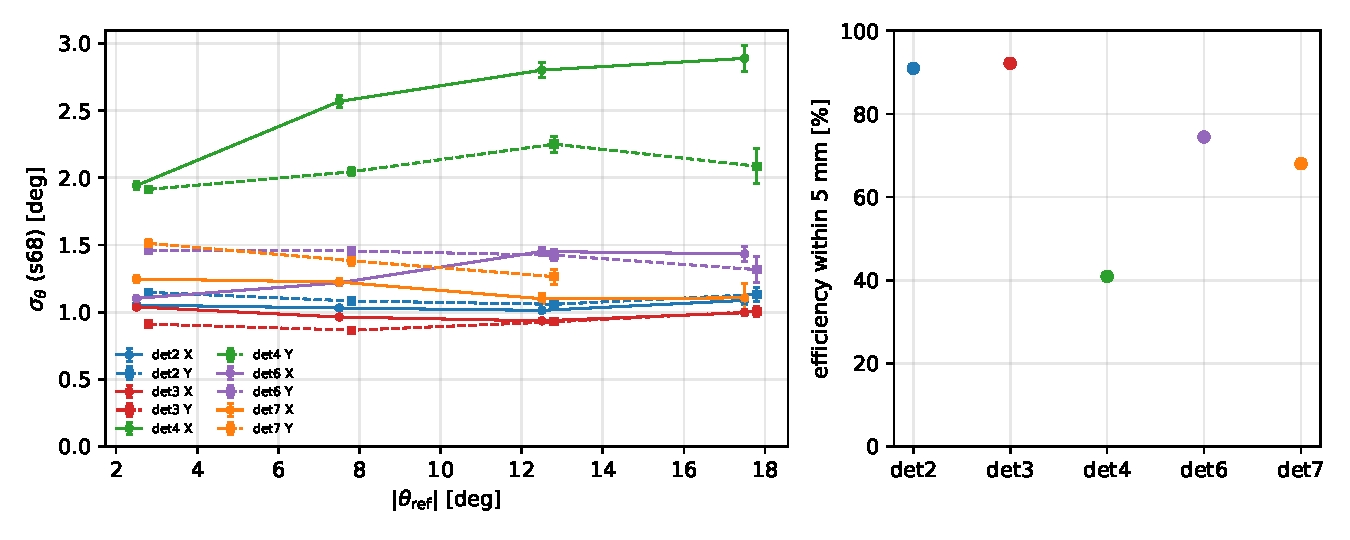
\includegraphics[width=0.85\linewidth]{tracking_perf}
  \caption{\tbw{Cosmic tracking performance, five chambers.}}
  \label{fig:trackperf}
\end{figure}

\subsection{Intrinsic resolution in the beam}
\tbw{det4 at SPS: $176\pm10$\,\textmu m $=0.30\times$ pitch, reference fitted out. The bench 0.6--0.7\,mm is
M3 pointing $\oplus$ $\sim$1.1\,mrad multiple scattering (arithmetic).}
\analysis{D6}{optional: bench resolution decomposed by measurement or simulation}
\begin{figure}[t]
  \centering
  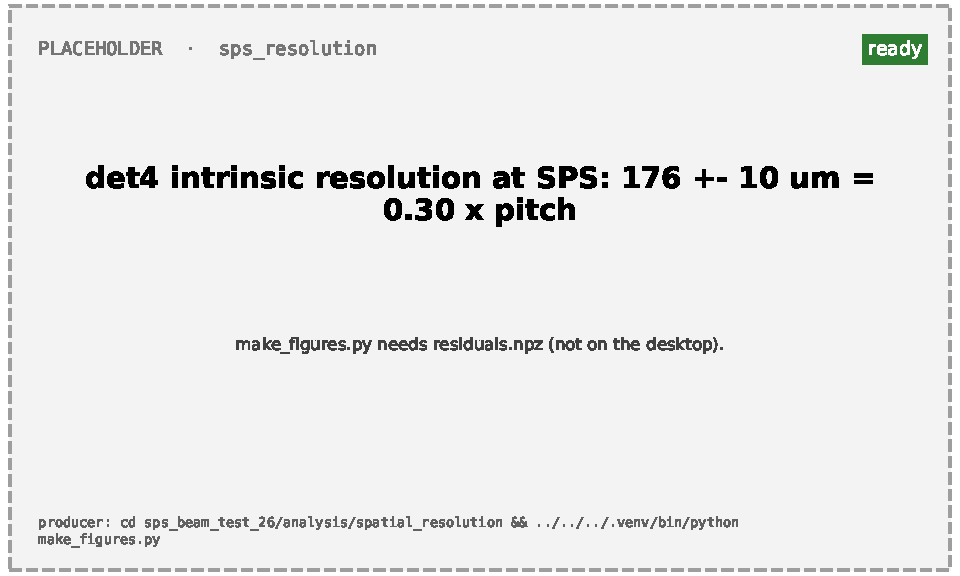
\includegraphics[width=0.7\linewidth]{sps_resolution}
  \caption{\tbw{det4 residual decomposition in the SPS beam.}}
  \label{fig:spsres}
\end{figure}
